\chapter{\gls{ide}}\label{cha:IDEs}

During programming tasks developers often interact with a variety of facilities and tools: browsers, \gls{ide}s, mail clients, virtual machines, etc. All these interactions are of high significance when it comes to understand the workflow of a developer. An \gls{ide} is very personal and therefore analysing developers' behavior is feasible. 

This chapter begins with an introduction to the history of \gls{ide}s to support their importance and a description of their future is given. Further, the main focus is the analysis and discussion of possible interaction with today's \gls{ide}s.

\section{Quick \gls{ide} History}

An \gls{ide} is a software application which aims to improve developers' productivity by facilitating application development. It consolidates the basic tools developers need to write and test software. Typically, an \gls{ide} consists of a source code editor, a compiler, a debugger and build automation tools. According to \addref{reference:} 
%https://www.veracode.com/security/integrated-development-environments} 
the idea behind \gls{ide} was realeased as Turbopascal which integrated an editor and a compile. However many believe Microsoft's Visual Basic (VB), launched in 1991 was the first real \gls{ide}, and by the time it was relatively easy to learn and use.

Over the years several \gls{ide}s have been implemented and released. \gls{ide}s offered remarkable advantages to developers mentioned in \addref{reference:}
% https://www.veracode.com/security/integrated-development-environments} 
and \addref{reference:} for example: %\addref{http://vantageonesoftware.com/advantages-disadvantages-integrated-development-environment/} for example: 
\begin{itemize}
\item Reducing the setup up time required to configure multiple development tools, 
\item Increasing development speed and efficiency by providing instant feedback for syntax errors or code insights,
\item Increasing program management by organising resources, providing a virtual representation of the project, and automatically adding appropriate imports. 
\item Increasing the quality of programs by offering the ability for debugging, testing and source control.
\end{itemize}


Overal these advantages of using an \gls{ide} have endorsed the productivity of a developer. Today, according to the Top IDE index \addref{reference:github}
%https://pypl.github.io/IDE.html}
, a ranking created by analysing how often \gls{ide}s are searched on Google, the 3 most used tools employed to develop source code are Eclipse, Visual Studio, Android Studio. Although \gls{IDE}s are stricking through the top 3, it is noticable that a significant amount of developers prefer to use highly configurable text editors such as Vim and Sublime Text. The different types of code, specific languages, cloud based, mobile application, apple or microsoft development, led \gls{ide}s to expand in a variety of directions. Consequently not all \gls{ide}s offer the same capabilities and the same collection of tools. Therefore one must be selective when choosing an \gls{ide}, in accordance to its development task and requirements. 

Even though that \gls{ide}s are highly helpful to a developer, they lack effective support to browse between complex relationships between source code elements. This implies that developers spend 30\% their time navigating through a chaotic environment and therefore their productivity is being reduced as supported by \addref{Taming the IDE with Fine-grained Interaction Data}. \addref{Autumn leaves} and \addref{An explatory study}

%D. Roethlisberger, O. Nierstrasz, and S. Ducasse, Autumn leaves:
%Curing the window plague in IDEs, in Proceedings of WCRE (16th
%Working Conference on Reverse Engineering), 2009, pp. 237–246.} 

%{A. J. Ko, B. A. Myers, M. J. Coblenz, and H. H. Aung, An exploratory study of how developers seek, relate, and collect relevant information
%during software maintenance tasks, IEEE Transactions on Software Engineering, vol. 32, no. 12, pp. 971–987, 2006.}.


For this thesis, in an attempt to understand the developers' workflow the extraction of user interactions with an \gls{ide} is required. The decision to analyse and develop for Eclipse \gls{ide} was taken for a vast amount of reasons listed in \ref{cha:TheEclipseIDE}.



\section{Interactions within \gls{ide}}

\gls{ide}s are highly used by developers nowadays to develop and maintain a software. Developers use \gls{ide} to read, navigate, understand and write code. In more detail the developer interacts with \gls{ide} through low level events such as: mouse clicks and keyboard shortcuts but also high level events facilitated by the tools provided in the toolbar such as: refactoring, debugging, navigating, testing, inspecting as mentioned in \addref{An explatory study}
and \addref{How Much Integrated Development Environments Improve Productivity}. 
%{A. J. Ko, B. A. Myers, M. J. Coblenz, and H. H. Aung, An exploratory study of how developers seek, relate, and collect relevant informationduring software maintenance tasks, IEEE Transactions on Software Engineering, vol. 32, no. 12, pp. 971–987, 2006.} 
A high level event is a series of low level events. In other words the toolbar allows the developer to code, compile and execute source code without having to follow manually these steps.  An example is the process of renaming a class within a large project. \gls{ide} provides contextual menues enabling fast and efficient changes where otherwise a series of low level events: editing several classes, compiling and error seeking, executing and testing the correctness after the change should be done manually.

	\begin{figure}[!ht]
		\begin{center}
		 
        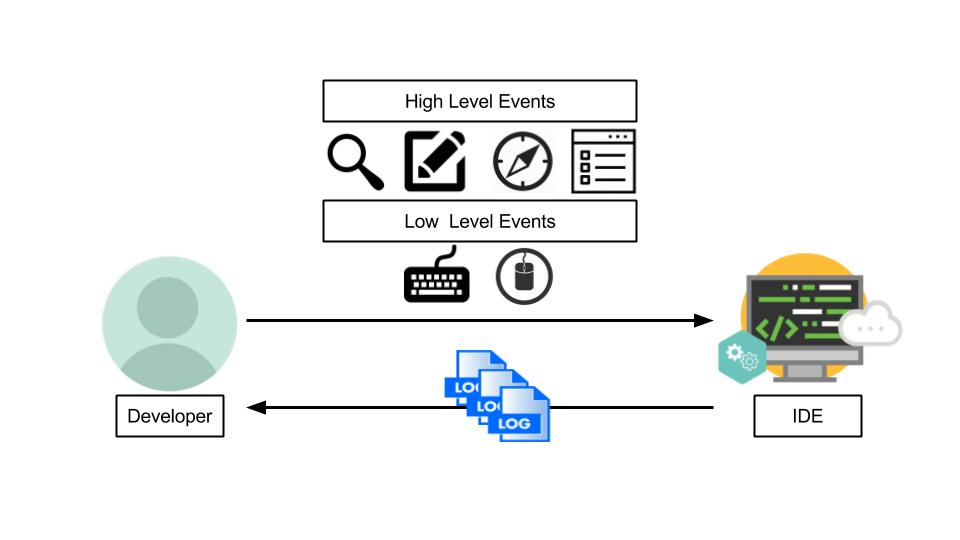
\includegraphics[width=\textwidth]{figures/ch1a_dev_ide.jpg}
		\end{center}
		\caption{Flow of usage data between developer and \gls{ide}.}
		\label{fig:ch1a_dev_ide}
	\end{figure}

According to \addref{Visualizing the Workflow of Developers} and \addref{Capturing and Exploiting IDE Interactions} by gathering all the IDE usage data provides an additional view of what the workflow of a developer is to solve a certain task.
A task (implementing a class, correcting an error) is consisting of a series of high and low level events  These interaction events are called usage data \addref{A Practical Guide to Analyzing IDE Usage Data} and they are an essential element for this thesis. All the usage data generated by the activity of a developer within an \gls{ide} are recorded. The developer initiates the different interactions and \gls{ide} responds back with logging particular events. The model in \ref{fig:ch1a_dev_ide} shows the exchange of usage data between developer and \gls{ide}.

\section{The usage data model} 
